
\begin{frame}
  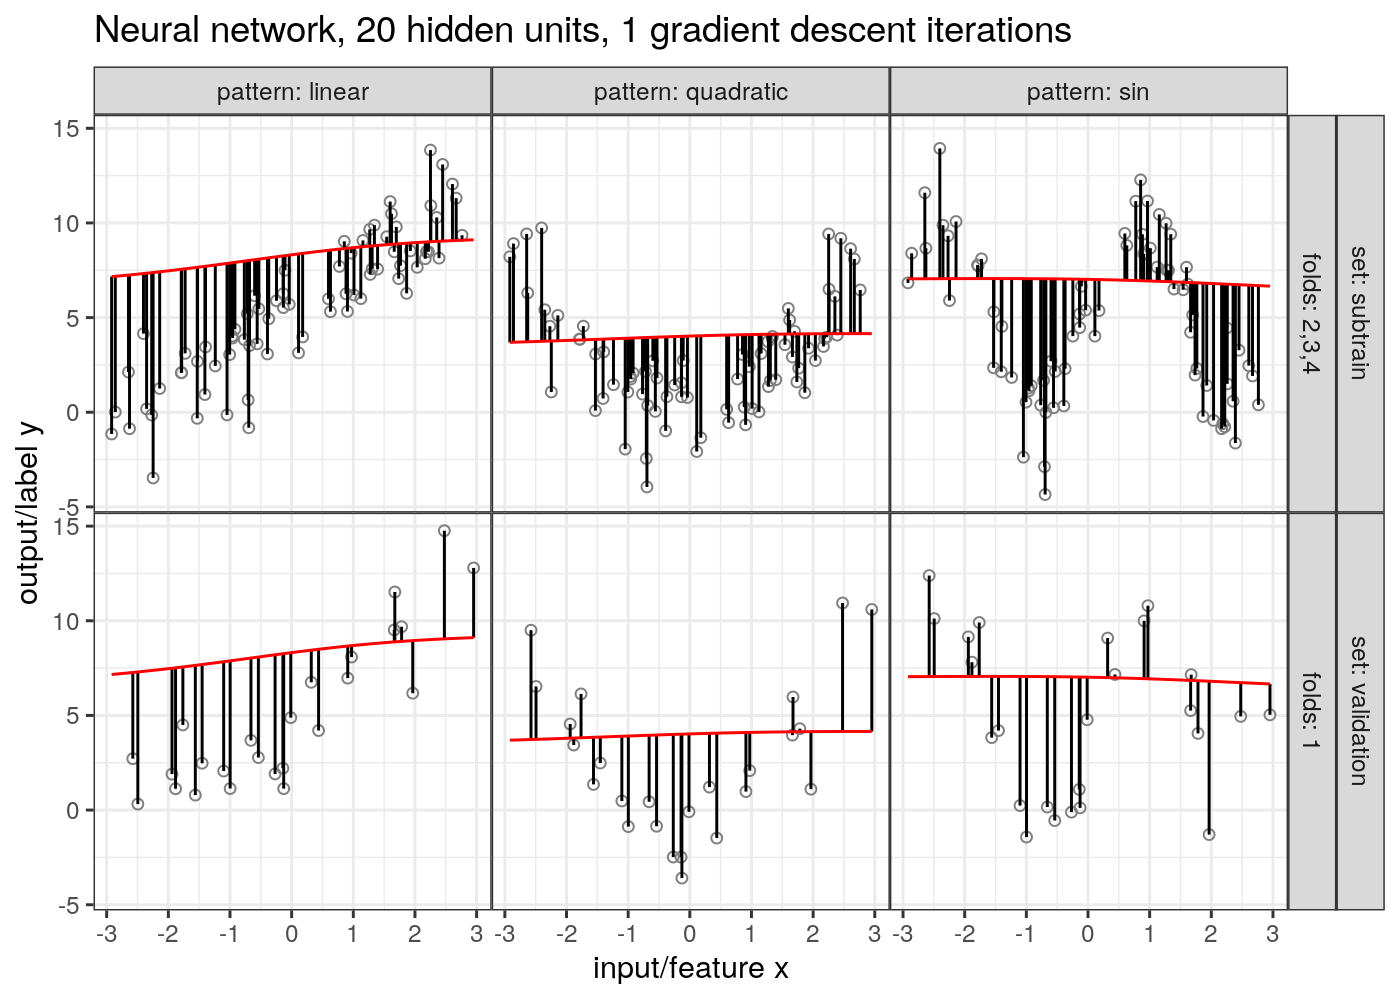
\includegraphics[width=\textwidth]{figure-overfitting-pred-units=20-maxit=1.png}
\ Data=grey dots, predictions=red curve, loss=black line segments.

\end{frame}


\begin{frame}
  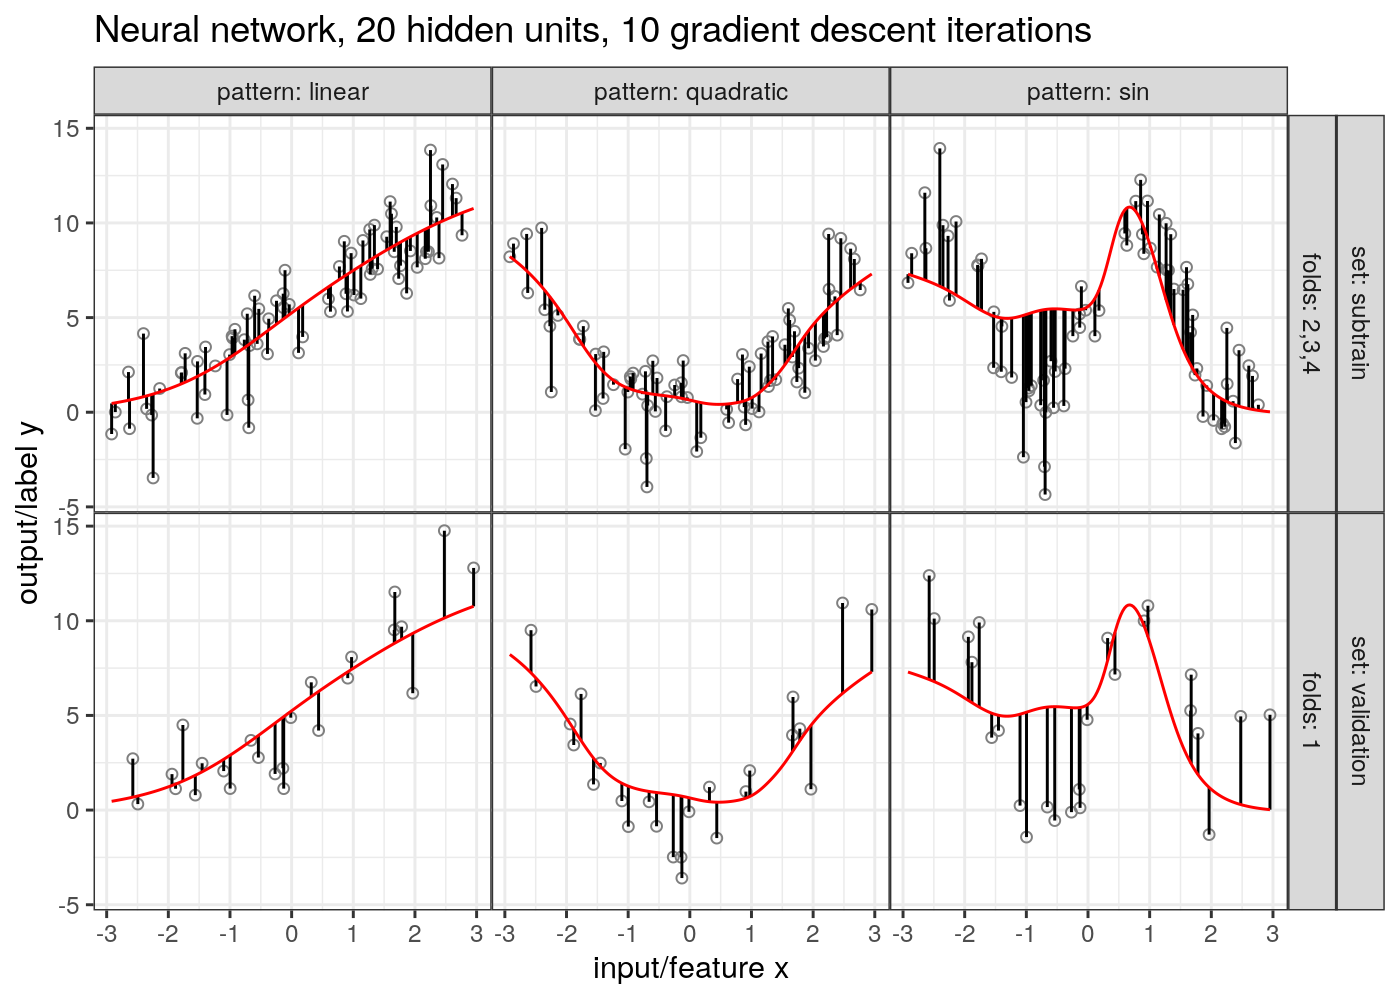
\includegraphics[width=\textwidth]{figure-overfitting-pred-units=20-maxit=10.png}
\ Data=grey dots, predictions=red curve, loss=black line segments.

\end{frame}


\begin{frame}
  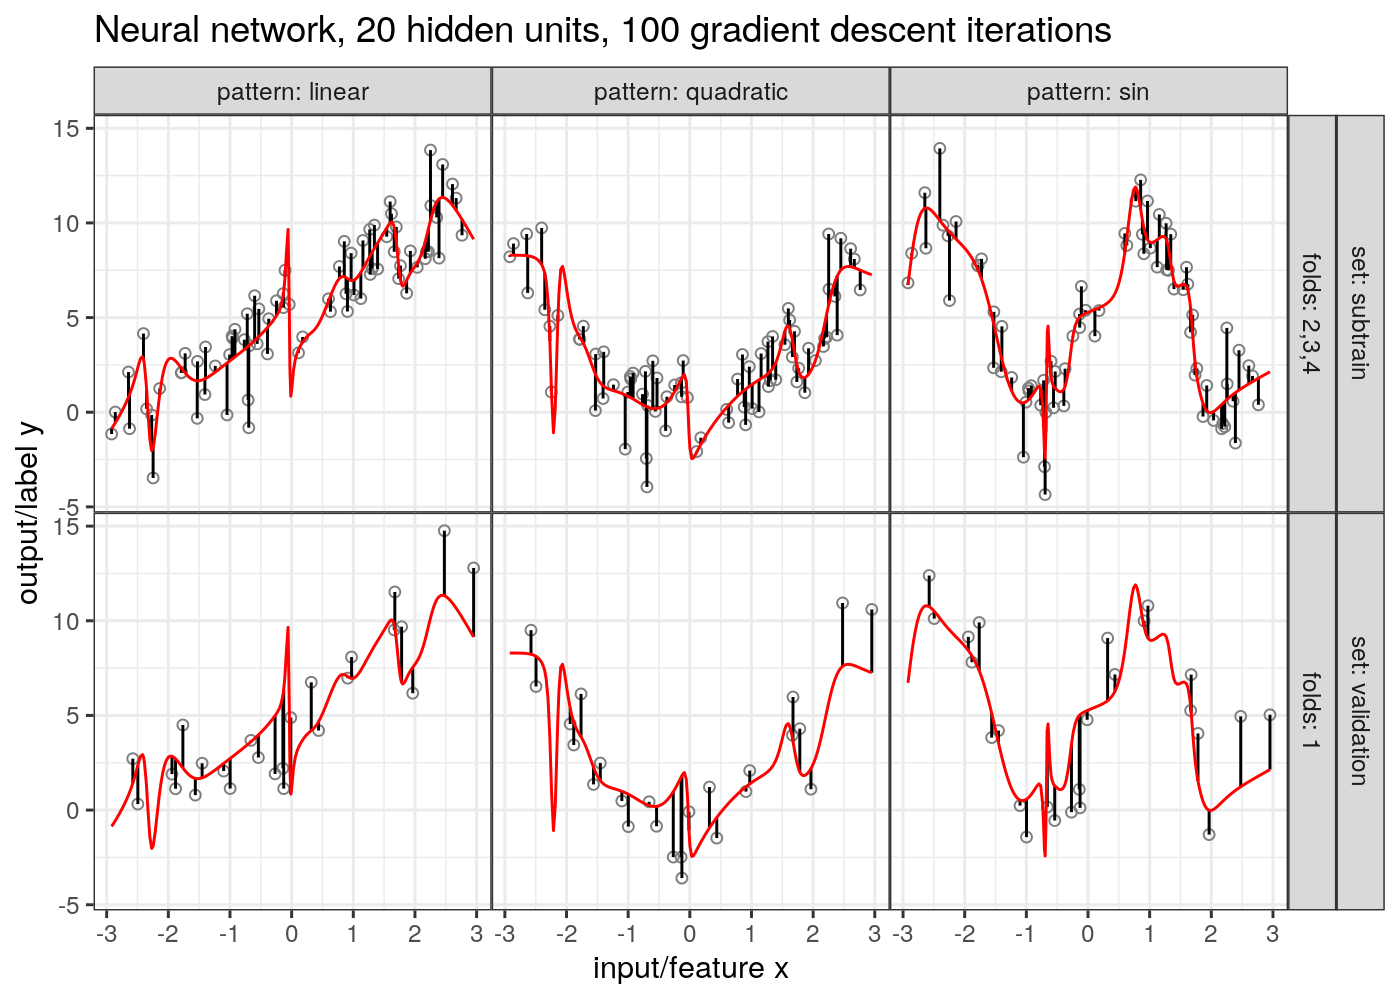
\includegraphics[width=\textwidth]{figure-overfitting-pred-units=20-maxit=100.png}
\ Data=grey dots, predictions=red curve, loss=black line segments.

\end{frame}


\begin{frame}
  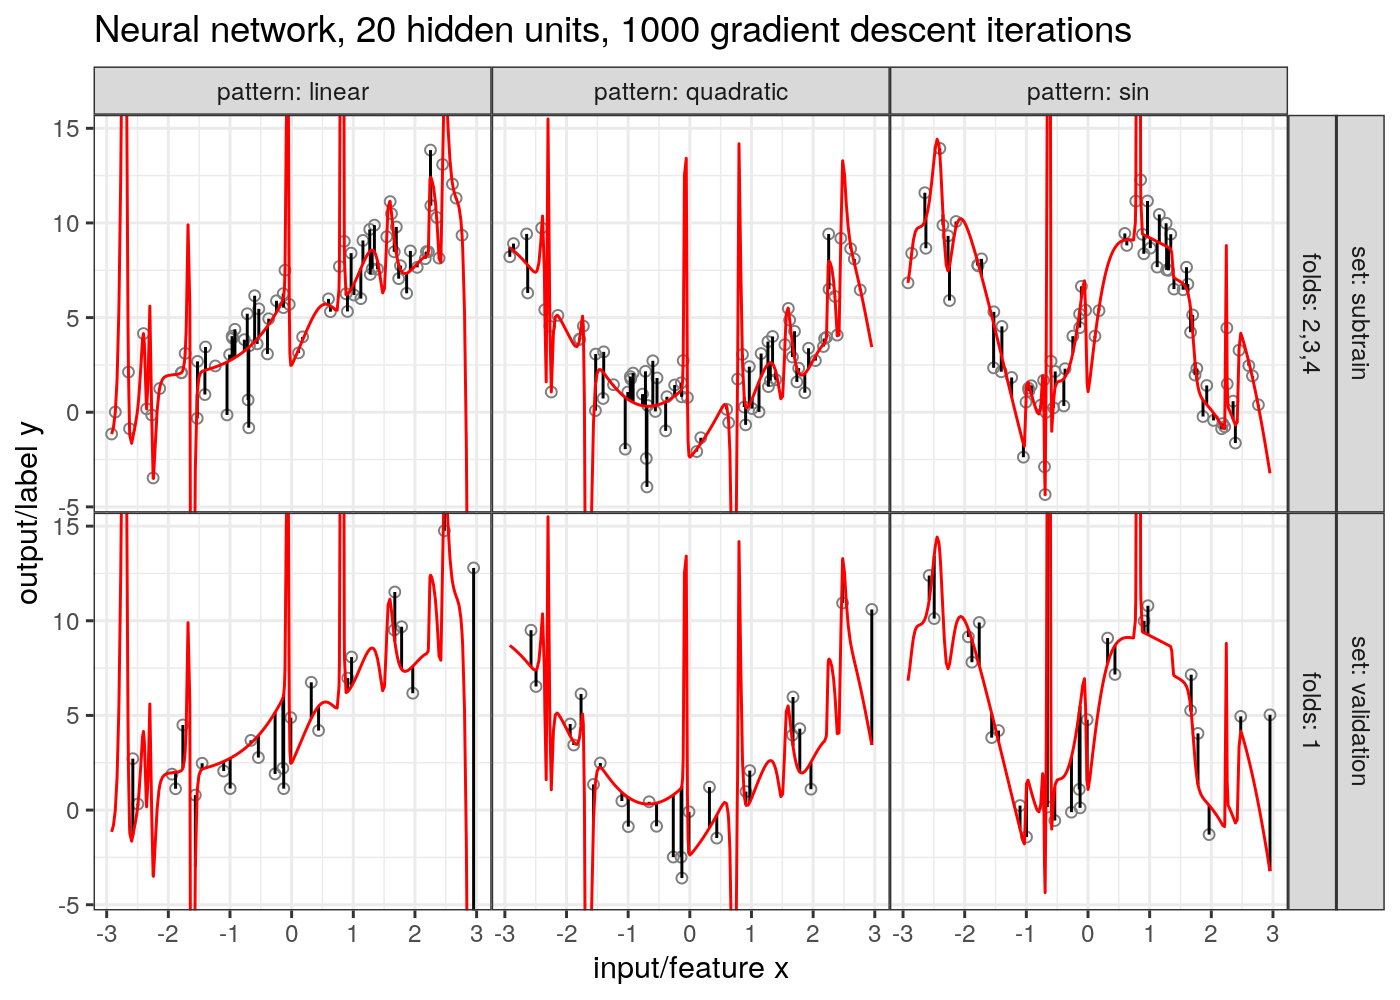
\includegraphics[width=\textwidth]{figure-overfitting-pred-units=20-maxit=1000.png}
\ Data=grey dots, predictions=red curve, loss=black line segments.

\end{frame}


\begin{frame}
  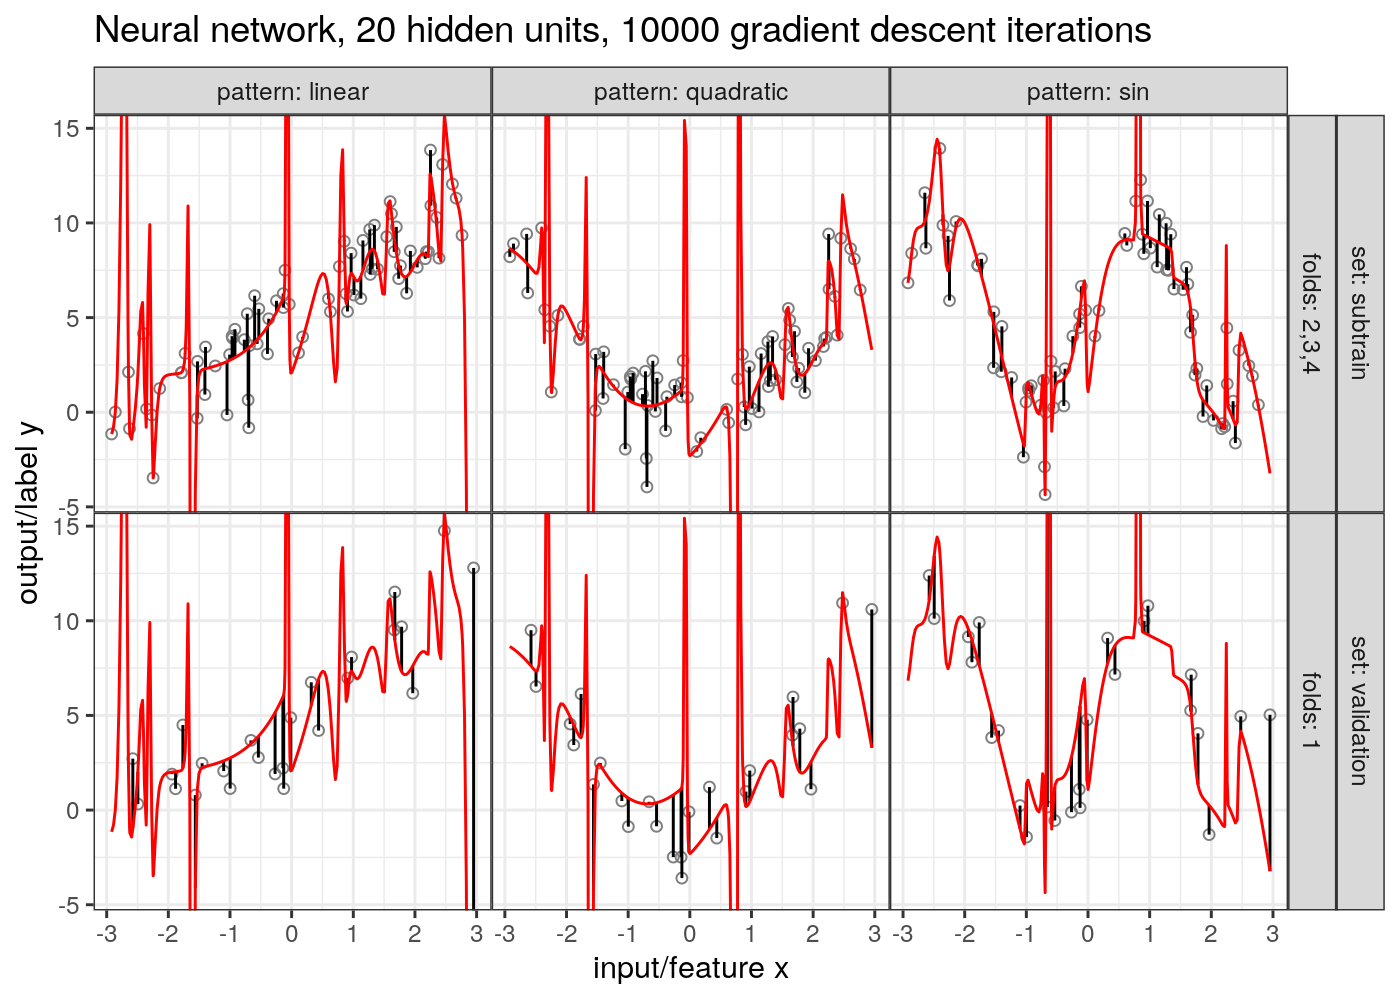
\includegraphics[width=\textwidth]{figure-overfitting-pred-units=20-maxit=10000.png}
\ Data=grey dots, predictions=red curve, loss=black line segments.

\end{frame}


\begin{frame}
  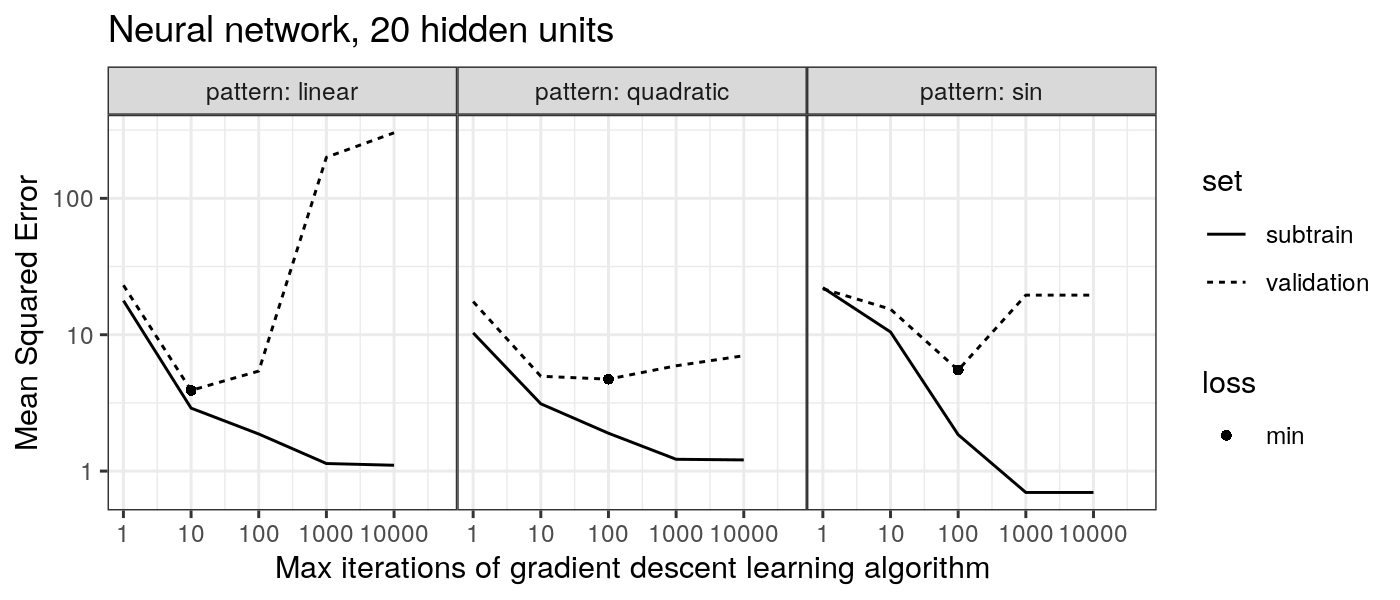
\includegraphics[width=\textwidth]{figure-overfitting-data-loss-20.png}
Different number of iterations best for different data.
\end{frame}

